\style{ft}
%   Titre de la sous section
\section{Mémo : les blocs principaux \mb}

%   colonne de gauche
\begin{minipage}[t]{0.75\linewidth}

    \begin{blocBase}\\
      \rule{-0.25em}{2em}
      Dans cette catégorie, on trouve les deux blocs essentiels qui sont d'ailleurs présents par défaut à l'ouverture d'un nouveau projet.

      \begin{itemize}
        \item Le bloc "au démarrage" permet d'initialiser un programme, la séquence d'instruction qui y sera placée ne sera donc exécuté qu'une seule fois.
        \item   Le bloc "toujours" contient la séquence d'instruction qui sera perpétuellement exécutée par le processeur.
        \item Outre ces blocs, vous trouverez dans cette catégorie les éléments permettant d'afficher des figures, du texte, d'effacer l'écran, de faire une pause, etc ...
      \end{itemize}

    \end{blocBase}

\end{minipage}
%   petit "ressort"
%   pour centrer les 2 colonnes
\hfill
%   colonne de droite
\begin{minipage}[t]{0.25\linewidth}~\\
\vspace{5mm}

  	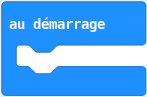
\includegraphics[scale=0.4]{res/blocsMkCd/MB_makecode_audemarrage.png}\\[0.5em]
  	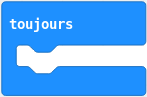
\includegraphics[scale=0.4]{res/blocsMkCd/MB_makecode_toujours.png}\\[0.5em]
    
\includegraphics[scale=0.4]{res/blocsMkCd/MB_makecode_base-icone.png}\\[0.5em]
    
\includegraphics[scale=0.4]{res/blocsMkCd/MB_makecode_base-texte.png}\\[0.5em]
    
\includegraphics[scale=0.4]{res/blocsMkCd/MB_makecode_base-pause.png}


\end{minipage}



%%%% Entrées
%   colonne de gauche
\begin{minipage}[t]{0.75\linewidth}

    \begin{blocEntrees}\\
      \rule{-0.25em}{2em}
La catégorie "Entrées" proposent notamment des blocs "Lorsque" qui fonctionnent de la même façon que le bloc "Toujours", à la différence que le \mb est ici en perpétuelle attente d'un évènement, que ce soit l'appui sur un bouton, un geste ou l'activation d'une broche.\\
\vspace{5mm}
On y trouve aussi les blocs permettant de recueillir les données :
\begin{itemize}
  \item savoir si un bouton est pressé;
  \item connaître la mesure de l'accélération;
  \item relever la température (du processeur);
\end{itemize}

    \end{blocEntrees}

\end{minipage}
%   petit "ressort"
%   pour centrer les 2 colonnes
\hfill
%   colonne de droite
\begin{minipage}[t]{0.25\linewidth}~\\
  \vspace{5mm}

    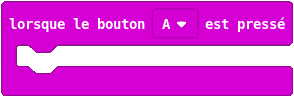
\includegraphics[scale=0.4]{res/blocsMkCd/MB_makecode_entrees-bouton.png}\\[0.5em]
    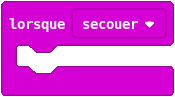
\includegraphics[scale=0.4]{res/blocsMkCd/MB_makecode_entrees-geste.png}\\[0.5em]
    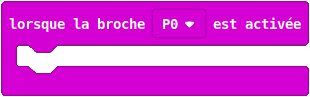
\includegraphics[scale=0.4]{res/blocsMkCd/MB_makecode_entrees-broche.png}\\[0.5em]
    
\includegraphics[scale=0.4]{res/blocsMkCd/MB_makecode_entrees-boutonPress.png}\\[0.5em]
    
\includegraphics[scale=0.4]{res/blocsMkCd/MB_makecode_entrees-accel.png}\\[0.5em]
    
\includegraphics[scale=0.4]{res/blocsMkCd/MB_makecode_entrees-temp.png}


\end{minipage}

%%%%

%%%%blocRadio
%   colonne de gauche
\begin{minipage}[t]{0.75\linewidth}

    \begin{blocRadio}\\
      \rule{-0.25em}{2em}
      Les fonctions de communication du \mb se trouve dans cette catégorie.\\
      Les données envoyées (nombre et/ou chaîne de caractères) ne sont pas "routées" : les reçoivent qui peut. Pour filtrer les réceptions il est possible de définir des groupes.\\
      \vspace{5mm}
      Les blocs de "réception" se comportent comme des blocs d'entrées et attendent perpétuellement un événement.


    \end{blocRadio}

\end{minipage}
%   petit "ressort"
%   pour centrer les 2 colonnes
\hfill
%   colonne de droite
\begin{minipage}[t]{0.25\linewidth}~\\
  \vspace{5mm}

    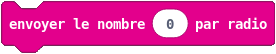
\includegraphics[scale=0.4]{res/blocsMkCd/MB_makecode_radio-envoyer.png}\\[0.5em]
    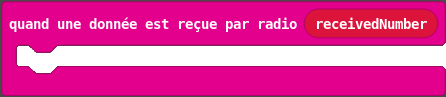
\includegraphics[scale=0.3]{res/blocsMkCd/MB_makecode_radio-recevoir.png}\\[0.5em]


\end{minipage}
%%%%

%%%% boucles
%   colonne de gauche
\begin{minipage}[t]{0.75\linewidth}

    \begin{blocBoucle}\\
      \rule{-0.25em}{2em}
      Cette catégorie contient les blocs permettant de faire des boucles ils sont aux nombres de 4 :

      \begin{itemize}
        \item "répéter", qui est le plus simple et qui convient dans un grand nombre de cas;
        \item  "tant que", qui répète la séquence tant que la condition indiquée est vraie;
        \item "pour" qui répète une séquence en incrémentant une valeur entière ou un index de liste;
      \end{itemize}

    \end{blocBoucle}

\end{minipage}
%   petit "ressort"
%   pour centrer les 2 colonnes
\hfill
%   colonne de droite
\begin{minipage}[t]{0.25\linewidth}~\\
  \vspace{5mm}


  	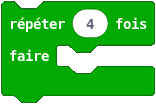
\includegraphics[scale=0.4]{res/blocsMkCd/MB_makecode_boucles-repeter.png}\\[0.5em]
  	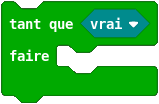
\includegraphics[scale=0.4]{res/blocsMkCd/MB_makecode_boucles-tantque.png}\\[0.5em]
    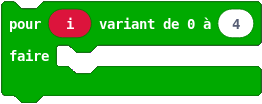
\includegraphics[scale=0.4]{res/blocsMkCd/MB_makecode_boucles-parcourir.png}


\end{minipage}

%%%%

%%%%blocLogique
%   colonne de gauche
\begin{minipage}[t]{0.75\linewidth}

    \begin{blocLogique}\\
      \rule{-0.25em}{2em}
      Dans la catégorie "Logique" nous allons trouver les blocs relatifs aux instructions conditionnelles, aux tests et au booléens\\

      \begin{itemize}
        \item Les blocs conditionnels permettent d'exécuter une suite d'instruction si le résultat d'un test donné est vrai.On modifie le nombres de conditions en cliquant sur + ou -.
        \item Les blocs de test permettent de comparer des nombres, des chaînes de caractères, des booléens...
        \item Les blocs booléens permettent d'effectuer des opérations logiques.
      \end{itemize}

    \end{blocLogique}

\end{minipage}
%   petit "ressort"
%   pour centrer les 2 colonnes
\hfill
%   colonne de droite
\begin{minipage}[t]{0.25\linewidth}~\\
  \vspace{5mm}

    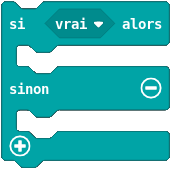
\includegraphics[scale=0.4]{res/blocsMkCd/MB_makecode_logique-sisinon.png}\\[0.5em]
    
\includegraphics[scale=0.4]{res/blocsMkCd/MB_makecode_logique-test.png}\\[0.5em]
    
\includegraphics[scale=0.4]{res/blocsMkCd/MB_makecode_logique-bool.png}

\end{minipage}
%%%%

%%%%blocVariable
%   colonne de gauche
\begin{minipage}[t]{0.75\linewidth}

    \begin{blocVariable}\\
      \rule{-0.25em}{2em}
      Par défaut, cette catégorie est vide tant qu'aucune variable n'a été définie, ou qu'aucun bloc comprenant une variable par défaut n'a été utiliser.\\
      Une variable peut bien sûr contenir un nombre, un booléen, une chaîne de caractères, une liste...

      \begin{itemize}
        \item Le bloc "définir" permet d'affecter une valeur à la variable.
        \item Le bloc "changer par" consisite à incrémenter la valeur de la variable
      \end{itemize}

    \end{blocVariable}

\end{minipage}
%   petit "ressort"
%   pour centrer les 2 colonnes
\hfill
%   colonne de droite
\begin{minipage}[t]{0.25\linewidth}~\\
  \vspace{5mm}

    
\includegraphics[scale=0.4]{res/blocsMkCd/MB_makecode_variables-variable.png}\\[0.5em]
    
\includegraphics[scale=0.4]{res/blocsMkCd/MB_makecode_variables-definir.png}\\[0.5em]
    
\includegraphics[scale=0.4]{res/blocsMkCd/MB_makecode_variables-incrementer.png}

\end{minipage}
%%%%

%%%%blocMaths
%   colonne de gauche
\begin{minipage}[t]{0.75\linewidth}

    \begin{blocMaths}\\
      \rule{-0.25em}{2em}
      Vous trouverez dans cette catégorie tous les blocs pour les opérations classiques, mais aussi les blocs permettant de générer de l'aléatoire, ou encore de contraindre ou mapper des valeurs.


    \end{blocMaths}

\end{minipage}
%   petit "ressort"
%   pour centrer les 2 colonnes
\hfill
%   colonne de droite
\begin{minipage}[t]{0.25\linewidth}~\\
  \vspace{5mm}

    
\includegraphics[scale=0.4]{res/blocsMkCd/MB_makecode_maths-aleaEntreBornes.png}\\[0.5em]
    
\includegraphics[scale=0.4]{res/blocsMkCd/MB_makecode_maths-aleaVraiFaux.png}\\[0.5em]
    
\includegraphics[scale=0.4]{res/blocsMkCd/MB_makecode_maths-mapper.png}\\[0.5em]


\end{minipage}
%%%%

%%%%blocFonctions
%   colonne de gauche
\begin{minipage}[t]{0.75\linewidth}

    \begin{blocFonctions}\\
      \rule{-0.25em}{2em}
      Pour accéder à cette catégorie, il faut dérouler le menu 
\includegraphics[scale=0.5]{res/blocsMkCd/MB_makecode_avance.png}.\\
      Tout comme pour la catégorie "Variables", il faut définir au préalable une fonction pour voir apparaître le bloc correspondant.\\
      \vspace{5mm}
      Une fonction peut être définie avec ou sans paramètres d'entrées.\\
      Une fonction en bloc ne renvoie pas de valeur.\\
      Une fois la fonction définie, on dispose d'un bloc pour l'appeler.


    \end{blocFonctions}

\end{minipage}
%   petit "ressort"
%   pour centrer les 2 colonnes
\hfill
%   colonne de droite
\begin{minipage}[t]{0.25\linewidth}~\\
  \vspace{5mm}

    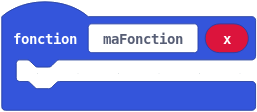
\includegraphics[scale=0.4]{res/blocsMkCd/MB_makecode_fonctions-definir.png}\\[0.5em]
    
\includegraphics[scale=0.4]{res/blocsMkCd/MB_makecode_fonctions-appeler.png}\\[0.5em]


\end{minipage}
%%%%
